\documentclass[final]{beamer}
\mode<presentation> {
    \usetheme{stanford}
}
\usepackage[english]{babel}
\usepackage[latin1]{inputenc}
\usepackage{citesupernumber}
\usepackage{wrapfig}
\usepackage{graphicx}
\usepackage{amsmath,amsthm, amssymb, latexsym, subfigure}
\newcommand{\subitem}[1]{\begin{itemize}\item #1 \end{itemize}}
\usefonttheme[onlymath]{serif}
%\boldmath

% 48 inches x 38 inches
\usepackage[orientation=landsSe,size=custom,width=91.44,height=91.44,scale=1.6,debug]{beamerposter}
\beamertemplategridbackground[1cm]

\title{Accelerated Sampling of Mutants: An MSM-based Hierarchical Bayesian Strategy}
\author{Robert McGibbon and Vijay Pande}
\institute[Stanford University]{Department of Chemistry, Stanford University, Stanford, CA.}
\date[Jun. 10, 2012]{Jun. 10, 2012}



\begin{document}
\begin{frame}{}%\begin{beamercolorbox}{structure}
  \vspace{-1.2in}
  \begin{columns}[t]

 %%%%%%%%%%%%%%%%%%%%%%%%%%%%%%%%%%%%%%%%%%%%%%%%%%%%%%%%%%%%%%%%%%%%%%%%%%%%%%%
% Column 1
%%%%%%%%%%%%%%%%%%%%%%%%%%%%%%%%%%%%%%%%%%%%%%%%%%%%%%%%%%%%%%%%%%%%%%%%%%%%%%%

\begin{column}{.3\linewidth}

\begin{block}{Introduction}
  \begin{itemize}
  % what am I doing
  \item Mutational analysis is the bread and butter of experimental protein biophysics.
  \item In simulations, mutational analysis is a major challenge, because the costs scale proportional to the number of mutants.
  \item Mutational analysis is \emph{useful} because of existence of extensive
  mutual information between mutants.
  \item This suggests that extensive simulations of a wild-type protein can be an \alert{informative prior} on new simulations of a mutant.
  \item Our Ansatz: mutation perturbs the rates of interconversion between a unknown subset of the conformational states of a protein.
  \end{itemize}
\end{block}
\vspace{0.5in}

\begin{block}{Model}
\begin{itemize}
    \item Use a common discretization of the state space between the mutant and wild type.

    \item Let $\vec{p_i}^{M}$ be the outbound transition probabilities from state $i$ in mutant, $\vec{c_i}^{WT}$ be the observed outbound transition counts from state $i$ in the wild type.

    \item Let the transfer coefficients, $q_i \in (0, 1)$, be the degree of information transfer between wildtype and mutant state $i$.

    \item \alert{Informative prior} on $\vec{p_i}^{MT}$:
    $$ \vec{p_i}^{MT} \sim \operatorname{Dirichlet}(q_i \cdot \vec{c_i}^{WT} + 1/2) $$
    %\item In the absence of new data, we expect the mutant to look like the wildtype.
    \item When $q_i=0$, we have Jeffreys prior, when $q_i > 0$, counts are \alert{inherited} from the wildtype into the mutant.
    
    \item $q_i$ must also be learned from the data. For convenience, the prior on $q_i$ is Beta, with shared hyperparameters, which constrains $q_i \in (0,1)$:
    $$ q_i \sim Beta(\alpha, \beta) $$
    \item Posterior distribution on $p_i$:
    \begin{align*}
    P(&\vec{p}_i^{MT} \vert \vec{c_i}^{MT}) \propto \\
    &\int_0^1 dq_i \; \operatorname{Dir}(q_i \cdot \vec{c}_i^{WT} + \vec{c_i}^{MT} + 1/2) \cdot  P_{\alpha, \beta}(q_i)
    \end{align*}
    
\end{itemize}
\end{block}
%end col1
\end{column}

%%%%%%%%%%%%%%%%%%%%%%%%%%%%%%%%%%%%%%%%%%%%%%%%%%%%%%%%%%%%%%%%%%%%%%%%%%%%%%%
% Column 2
%%%%%%%%%%%%%%%%%%%%%%%%%%%%%%%%%%%%%%%%%%%%%%%%%%%%%%%%%%%%%%%%%%%%%%%%%%%%%%%
\begin{column}{.3\linewidth}

\begin{block}{Methods}
\begin{itemize}
\item Our sampling principle: choose actions that maximize the model's \alert{expected information gain (EIG)}.

\item The actions considered are ``from which state shall I start further sampling?''

\item Conditional on $q_i$, the EIG of observing a ``count'', $e$, is given by the expected Kullbeck--Leibler divergence from the current posterior ,$P(\vec{p_i}^{MT} | q_i)$, to the updated posterior, $P(\vec{p_i}^{MT} | q_i, e)$.

$$
D_{KL}(P||Q) = \int_{-\infty}^{\infty} dx \ln\left( \frac{p(x)}{q(x)} \right) p(x)
$$

\item For Dirichlet distributions,
\begin{align*}
D_{KL}(\lambda^q &|| \lambda^p) = \log \frac{\Gamma(\lambda^{qt})}{\Gamma(\lambda^{pt})} + \sum_{s=1}^m \log \frac{\Gamma(\lambda^p_s)}{\Gamma(\lambda^q_s)} \\
&+ \sum_{s=1}^m \left[\lambda^q_s -\lambda^p_s\right]\left[\Psi(\lambda^q_s) - \Psi(\lambda^{qt})\right]
\end{align*}


\item If $e$ is a single count, distributed according to the current Dirichlet-Multinomial posterior, than this simplifies to

\begin{align*}
E[D_{KL} \vert q_i] &= \Psi(\lambda^t) - \log(\lambda^t) + \\
 &\frac{1}{\lambda^t} \sum_l \left[ \lambda_l \left( \log (\lambda_l) - \Psi(\lambda_l) \right) \right] 
\end{align*}

where $\lambda = q_i \cdot \vec{c}_i^{WT} + \vec{c_i}^{MT} + 1/2$ and $\Psi$ is the digamma function.

\item Still requires Markov chain Monte Carlo over $q_i$.

\end{itemize}
\end{block}
\vspace{1in}


\begin{figure}
    \centering
 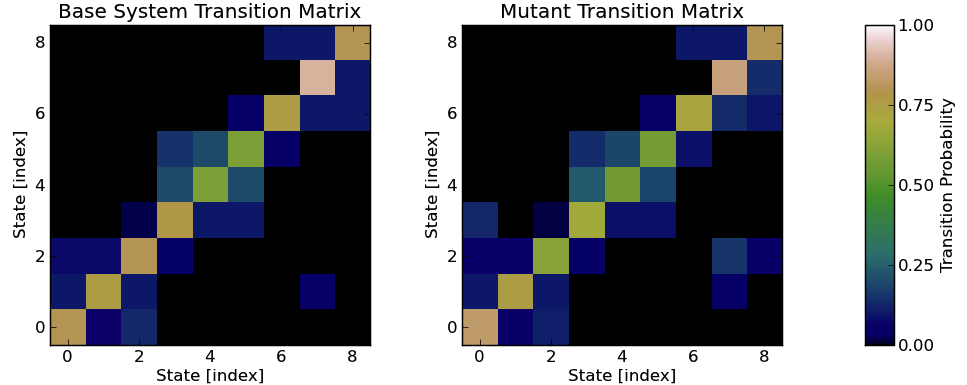
\includegraphics[width=\textwidth]{../code/9x9graph/plots/transition_matrices-tight.png}
    \caption{Transition probability matrix for an example system with nine states. Here, the mutant has new connections $3\rightarrow 0, 2\rightarrow 7, 2\rightarrow 8$}
\end{figure}


% \begin{minipage}
% \begin{figure}    
% 
% \end{figure}
% \end{minipage}



\end{column}
%%%%%%%%%%%%%%%%%%%%%%%%%%%%%%%%%%%%%%%%%%%%%%%%%%%%%%%%%%%%%%%%%%%%%%%%%%%%%%%
% Column 3
%%%%%%%%%%%%%%%%%%%%%%%%%%%%%%%%%%%%%%%%%%%%%%%%%%%%%%%%%%%%%%%%%%%%%%%%%%%%%%
\begin{column}{.3\linewidth}

\begin{block}{Example}
\end{block}

\begin{figure}
 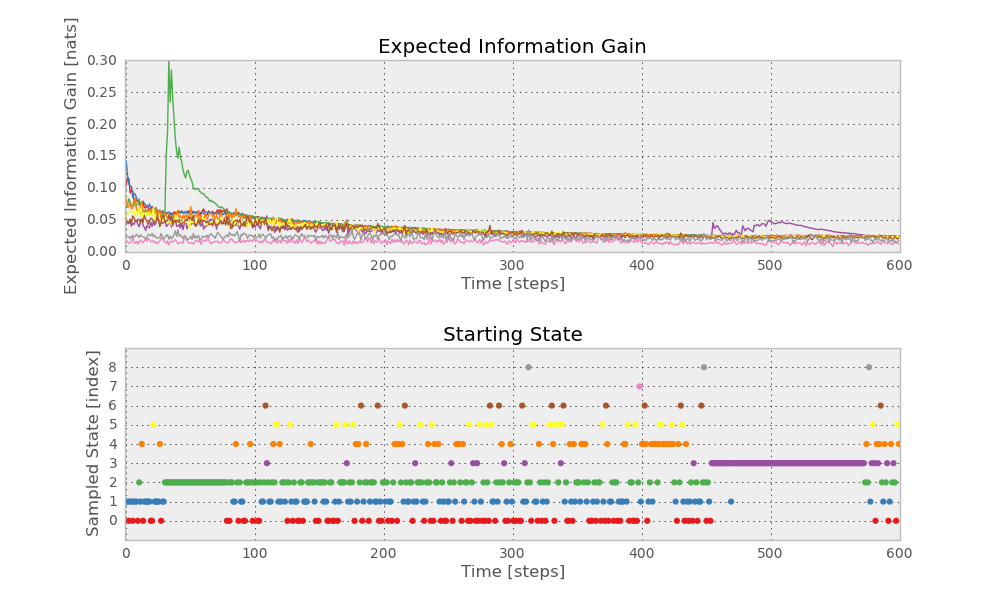
\includegraphics[width=\textwidth]{../code/9x9graph/plots/information_gain.png}
    \caption{When the model discovers unexpected behavior anomalies, like the transitions from $2$ and $3$, it focuses its sampling there.}
\end{figure}

\begin{figure}
 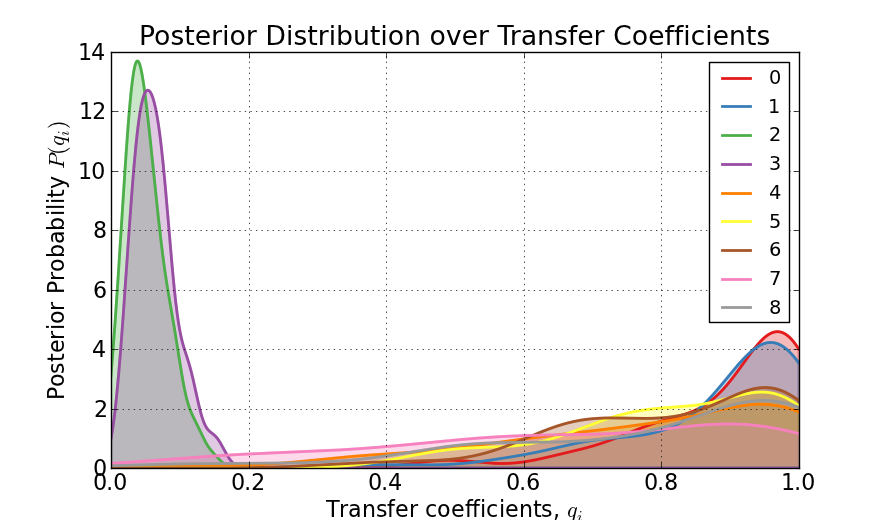
\includegraphics[width=\textwidth]{../code/9x9graph/posterior_q.png}
    \caption{The posterior distributions over $q$ show that the model has correctly ``discovered'' that states $2$, $3$ are dissimilar in the mutant. Some states (e.g. $8$) that are undersampled still feature very wide posteriors.}
\end{figure}


    
\begin{block}{Limitations}
\begin{itemize}
\item Conformational states are assumed to be the same for wildtype and mutant.
\item No model for reversibility or detailed balance constraints.
\item Uncertainty due to low wildtype counts in low-population unfolded microstates can swamp model, focus sampling there.
\end{itemize}
\end{block}
\vspace{0.5in}

% \begin{block}{Conclusions}
% \begin{itemize}
% \item We can focus sampling on the regions of phase space that appear different between the mutant and the wildtype, and bootstrap off our sampling of the wildtype when they appear similar.
% \end{itemize}
% \end{block}
% \vspace{0.5in}

\begin{block}{References}
\bibliographystyle{jacs-new}
\bibliography{Library.bib}
\footnotesize
\begin{itemize}
\item Patil, A.; Huard, D.; Fonnesbeck, C. J. ``PyMC: Bayesian stochastic modelling in Python.'' \emph{J. Stat. Softw.} 35 1 (2010)
\item Cohn, D; Atlas, L.; Ladner, R. ``Improving generalization with active learning.'' \emph{Machine Learning} 15 201 (1994)
\end{itemize}
\end{block}

\end{column}l
\end{columns}
\end{frame}
\end{document}
